\documentclass[times, utf8, zavrsni]{fer}
\usepackage{booktabs}
\usepackage{graphicx}
\graphicspath{{./images/}}

\begin{document}

% TODO: Navedite broj rada.
\thesisnumber{5672}

% TODO: Navedite naslov rada.
\title{Sustav za upravljanje i pretraživanje baze PDF dokumenata}

% TODO: Navedite vaše ime i prezime.
\author{Luka Čupić}

\maketitle

% Ispis stranice s napomenom o umetanju izvornika rada. Uklonite naredbu \izvornik ako želite izbaciti tu stranicu.
\izvornik

% Dodavanje zahvale ili prazne stranice. Ako ne želite dodati zahvalu, naredbu ostavite radi prazne stranice.
\zahvala{}

\tableofcontents

\chapter{Uvod}
Područje analize i pretraživanja teksta neizbježno je u današnjem svijetu tehnologije. Od internetskih tražilica koje pretražuju enormne količine podataka baziranih na zadanom upitu, osobnih pomoćnika na pametnim mobitelima koji procesiraju izgovorene riječi pa sve do analize i prepoznavanja \textit{spam} elektroničkih poruka.
Kratki osvrt na ove te mnoge druge primjene ukazuju na nepobitnu činjenicu da je pretraživanje teksta...

\chapter{Pregled područja}
Korištenje računala za povrat informacija (engl. \textit{information retrieval}) datira sve do četrdesetih godina dvadesetog stoljeća, daleko prije komercijalizacije računala, odnosno njihovog korištenja u osobne svrhe. Pogledamo li samo neke od relevantnih problema poput digitalizacije knjižnica i automatizacije knjižničnih poslova, statističku analizu tekstualnih podataka u svrhe X, procesiranje korisničkih upita kako bi se pronašli relevantni dokumenti, ... Očito je da je područje analize i pretraživanja teksta vrlo zastupljeno u današnjem digitalnom svijetu u kojem se količina informacija povećava za X posto svake godine (referenca na paper), očito je da je domena primjene vrlo široka te da su analiza i pretraživanje teksta praktički zastupljeni u svakom većem području koje iziskuje nekakvu vrstu analize i pretraživanja teksta odnosno povrata informacija.

\chapter{Model dokumenata}

\section{Prikaz dokumenata}
Prije \textit{poniranja u dubine}, objasnimo prvo što u kontekstu analize i pretraživanja teksta predstavlja dokument. Neformalno dokument možemo definirati kao kolekciju riječi. Ovakva kolekcija ne mora nužno biti skup, pošto dokument može imati više ponavljanja istih riječi (ova će činjenica doći do izražaja u \textbf{poglavlju X}). No ipak, za predstavljanje dokumenata biti će korišten tzv. \textit{model vreće riječi} (engl. \textit{bag of words model}) kod kojeg nam nije bitna semantika samih dokumenata, pa čak niti poredak riječi, već je bitna samo činjenica pojavljuju li se riječi u određenom dokumentu, odnosno koja je učestalost njihovog pojavljivanja.
Implementacija samog modela zamišljena je tako da se na početku iz svih dokumenata izvade sve riječi te potom uklone nebitne riječi (o kojima će više riječi biti kasnije) a od preostalih se riječi izgradi vektor koji će \textit{de-facto} predstavljati dokument. Najosnovniji prikaz dokumenata jest korištenjem binarne reprezentacije: od svih 
Ovakav model često je korišten u području procesiranja prirodnog jezika te povrata informacija kako iz dokumenata tako iz drugih izvora tekstualnih informacija.

Da bi se dokumenti mogli predstaviti u obliku vreća riječi, potrebno je odrediti vokabular—skup svih riječi koje se nalaze u svim dokumentima promatrane kolekcije dokumenata (u daljnjem tekstu: zbirka). Iz ovako zadanog vokabulara ćemo ponajprije, ukloniti sve zaustavne riječi (engl. \textit{stop words})—riječi koje su učestale u nekom jeziku te su stoga nebitne za sam postupak analize teksta. Primjeri nekih zaustavnih riječi u hrvatskom jeziku su: \textit{aha}, \textit{nešto}, \textit{okolo}, \textit{zaboga}. Osim zaustavnih riječi, dodatna obrada teksta može se obaviti tzv. \textit{stemanjem} (engl. \textit{stemming}). Ova metoda ima zadaću svesti riječi na njihov kanonski oblik. Drugim riječima, nebitno je je li riječ napisana u jednini ili množini ili pak u kojem je padežu; bitan je samo kanonski oblik riječi. Na primjer, riječi poput \textit{spavao} i \textit{spavati} biti će svedene na \textit{spavanje}.
Nakon stvaranja vokabulara te predobrade dokumenata (izbacivanje zaustavnih riječi, stemanje) možemo krenuti s predstavljanjem dokumenata. Radi praktičnosti, najčešća metoda predstavljanja dokumenata jest uz pomoć vektora.
Najjednostavnija metoda vektorskog predstavljanja dokumenata jest binarna: za svaku riječ iz vokabulara naprosto provjerimo nalazi li se u danom dokumentu te ukoliko se nalazi, odgovarajuća komponenta vektora (indeks riječi u vokabularu) biti će 1, a u suprotnom 0. Primjerice, ukoliko imamo dokumente $d_{1}$ = "Marko jako voli domaćice. Domaćice su dobre." te $d_{2}$ = "Marko voli domaćice i programiranje.", vokabular će nakon uklanjanja svih nebitnih znakova i stop riječi biti: V = {"Marko", "jako", "voli", "domaćice", "dobre", "programiranje"}. Koristeći binarnu metodu reprezentacije dokumenata, odgovarajući vektori će iznositi:
\begin{equation}
{{d_{1}}=[1, 1, 1, 1, 1, 0]}
\end{equation}
\begin{equation}
{{d_{2}}=[1, 0, 1, 1, 0, 1]}
\end{equation}
zbog toga što prvi dokument ne sadrži riječ "programiranje" dok drugi dokument ne sadrži riječ "jako".
Nadograđujući se na prethodnu metodu, dolazimo do frekvencijskog prikaza vektora. Umjesto obične binarne reprezentacije u kojoj pamtimo samo nalazi li se riječ u dokumentu ili ne, u frekvencijskom prikazu pamtimo i koliko se puta dotična riječ pojavljuje u dokumentu; komponente vektora zapravo su frekvencija (tj. broj) pojavljivanja određene riječi u dokumentu. Gledajući isti vokabular i dokumente kao u prethodnom primjeru, novi vektori će u ovom slučaju iznositi:
\begin{equation}
{{d_{1}}=[1, 1, 1, 2, 1, 0]}
\end{equation}
\begin{equation}
{{d_{2}}=[1, 0, 1, 1, 0, 1]}
\end{equation}
Primjećujemo da je jedina razlika u odnosu na prethodni primjer četvrta komponenta prvog vektora koja zapravo ukazuje na to da se riječ "domaćica" u prvom dokumentu pojavljuje dvaput.
Naposlijetku dolazimo i do najčešće metode vektorskog prikaza dokumenata — TF-IDF (engl. \textit{term frequency–inverse document frequency}). Ova metoda zasniva se na dvije intuitivne pretpostavke:
\begin{itemize}
\item[$\bullet$] riječ je važnija za semantiku dokumenta što se češće u njemu pojavljuje (TF komponenta)
\item[$\bullet$] riječ je manje važna za semantiku dokumenta što se češće pojavljuje u drugim dokumentima (IDF komponenta)
\end{itemize}
TF i IDF dakle predstavljaju dvije komponente vektora kojima ćemo predstavljati dokumente. Prva komponenta je već spomenuta, frekvencija pojavljivanja riječi \textit{w} u dokumentu \textit{d} — ($f_\textit{w, d}$) dok je druga komponenta obrnuta frekvencija pojavljivanja riječi u cijeloj zbirci.
Za riječ \textit{w} i dokument \textit{d}, TF i IDF komponene računaju se na sljedeći način:
\begin{equation}
{\displaystyle \mathrm {tf} (t,d)=f_{t,d}}
\end{equation}
\begin{equation}
{\displaystyle \mathrm {idf} (t,D)=\log {\frac {N}{|\{d\in D:t\in d\}|}}}
\end{equation}

Formula za TF komponentu je intuitivna i trivijalna. Formula za IDF komponentu zahtjeva kratki osvrt: riječ će biti bitnija za neki dokument što se rijeđe pojavljuje u drugim dokumentima. Odnosno drugim riječima: riječ će biti manje bitna za neki dokument što se češće pojavljuje u drugim dokumentima. Ovo ima smisla zato što neke riječi mogu biti česte u dokumentima čisto zbog same prirode jezika pa stoga ima smisla takve riječi manje uzimati u obzir prilikom računanja relevantnosti dokumenata. Dakle: što je riječ češća u ostalim dokumentima, IDF vrijednost se smanjuje te riječ postaje manje bitna za neki dokument. Naposlijetku, cijeli se omjer logaritamski skalira kako bi se u smanjio utjecaj velikog i/ili malog broja dokumenata koji sadrže određenu riječ.
TF-IDF EXAMPLE !!!

\section{Semantička sličnost dokumenata}
Nakon izgrađene vektorske reprezentacije svih dokumenata u korpusu, sljedeći korak jest samo uspoređivanje dokumenata. U sklopu ovog završnog rada, uspoređivanja dokumenata ostvaruje se na dva semantički različita načina: uspoređivanje korisničkog unosa (engl. \textit{user input}, \textit{query}) sa zbirkom dokumenata ili uspoređivanje dokumenta sa zbirkom dokumenata.
Ova dva, naizgled različita problema, zapravo se svode na jedan: uspoređivanje kolekcije riječi sa zbirkom dokumenata. Ideja je dakle sljedeća: gleda se koliko riječi (bilo iz korisničkog unosa, bilo iz dokumenta, u daljnjem razmatranju - ulazni vektor) iz ulaznog vektora odgovara riječima iz vokabulara, tj. koliko riječi iz ulaznog vektora odgovaraju riječima iz pojedinih dokumenata u zbirci. Što je veća korespondencija određenog ulaznog vektora s vektorom pojedinog dokumenta (tj. što više riječi dijele zajedno), to kažemo da su ta dva dokumenta sličnija. Primjerice, ukoliko se u zbirci nalazi dokument o srednjevjekovnoj povijesti, a kao ulazni vektor dovedemo neku srednjevjekovnu frazu, to će ulazni vektor i taj dokument imati veću mjeru sličnosti - što nas dovodi do same definicije.
Mjeru sličnosti (engl. \textit{document similarity}) definiramo kao vrijednost na skupu pozitivnih realnih brojeva, koja ukazuje na to koliko su dva dokumenta slična — što je brojka veća, dokumenti su sličniji.
U nastavku ćemo razmotriti metode mjere sličnosti korištene u ovome radu.

\subsection{Metoda kosinusne sličnosti}
Kako su dokumenti zapravo predstavljeni vektorima u više-dimenzijskom prostoru, nad takvim dokumentima (odnosno njihovim vektorima), možemo primijenjivati operacije linearne algebre, odnosno vektorske operacije. Počevši od definicije skalarnog umnoška dvaju vektora
\begin{equation}
\mathbf {a} \cdot \mathbf {b} =\left\|\mathbf {a} \right\|\left\|\mathbf {b} \right\|\cos \theta,
\end{equation}
dolazimo do mjere kosinusne sličnosti dvaju vektora (dokumenata):
\begin{equation}
{\text{similarity}}=\cos(\theta )={\mathbf {A} \cdot \mathbf {B}  \over \|\mathbf {A} \|\|\mathbf {B}}
\end{equation}
Dakle, sličnost dvaju dokumenata u ovom kontekstu prikazujemo kao kosinus kuta između njihovih vektora. Što su dokumenti sličniji, kosinus kuta biti će bliži jedinici, odnosno što su dokumenti različitiji, kosinus kuta biti će bliži nuli. Intuicija ovoga je sljedeća: ukoliko radi jednostavnosti zamislimo da vektori imaju samo dvije dimenzije te da nad njima radimo skalarni produkt, tada će sličnost dokumenata koje predstavljaju biti to veća što su oni "bliži" u koordinatnom sustavu, tj. što je kosinus njihovog kuta manji; vrijedi i da će dokumenti biti manje slični što je kosinus kuta njihovih vektora veći. SLIJEDI SLIKA

\begin{figure}
\makebox[\textwidth]{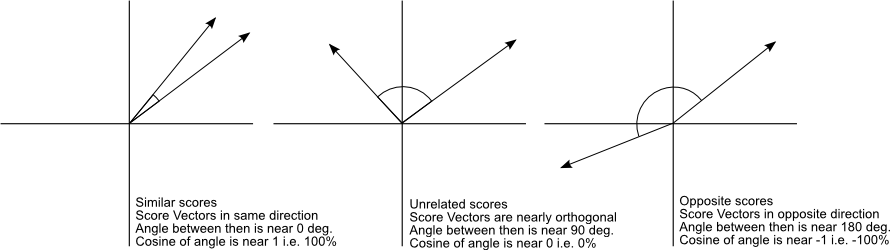
\includegraphics[width=\textwidth]{vectors.png}}
\caption{Prikaz sličnosti dvaju vektora u 2D koordinatnom sustavu}
\end{figure}

Ovo saznanje o kosinusnoj mjeri sličnosti dokumenata možemo iskoristiti u izgradnji sljedećeg modela: Neka je $v_{d_i}$ vektorska reprezentacija (binarna, frekvencijska ili TF-IDF) dokumenta $d_{i}$. Tada se sličnost dvaju dokumenata mjeri kao:
\begin{equation}
{\displaystyle {\text{similarity}}(d_{i}, d_{j})}={\frac{v_{d_i} \cdot v_{d_j}}{||v_{d_i}|| \cdot ||v_{d_j}||}}
\end{equation}
Pošto se skalarni produkt dva vektora svodi na sumu umnožaka pripadajućih komponenti (prva s prvom, druga s drugom itd.), ovo intuitivno možemo zamisliti tako da naprosto zbrajamo "korespondencije" odgovarajućih riječi. Naime, ako se riječ nalazi u oba dokumenta, tada će taj umnožak biti pozitivan te će se pridodati mjeri sličnosti, odnosno povećati ju. Ako neka riječ ne postoji u dokumentu, tada će taj umnožak biti nula pa će automatski sličnost biti manja.

\subsection{Metoda Okapi BM25}
Za razliku od metode kosinusne sličnosti, BM25 je funkcija rangiranja koja ima za zadaću direktno rangirati dokumente po relevantnosti određenom korisničkom upitu. Iako na prvi pogled ove dvije metode izgledaju različito, zapravo se svode na istu stvar pošto je dokument zapravo samo poopćeni oblik korisnikovog upita (više o tome u poglavlju s implementacijom).
Za dokument $Q$, koji sadrži riječi $q_{1}$,...,$q_{n}$, BM25 mjera sličnosti nekog dokumenta $D$ iz zbirke računa se kao:
\begin{equation}
{\displaystyle {\text{score}}(D,Q)=\sum _{i=1}^{n}{\text{IDF}}(q_{i})\cdot {\frac {f(q_{i},D)\cdot (k_{1}+1)}{f(q_{i},D)+k_{1}\cdot \left(((1-b+b\cdot {\frac {|D|}{\text{avgdl}}}\right)}},}
\end{equation}
gdje je ${\displaystyle f(q_{i},D)}$	 frekvencija od ${\displaystyle q_{i}}$ u dokumentu D, ${\displaystyle |D|}$ je broj riječi u dokumentu D, a avgdl je prosječan broj riječi u dokumentima iz zbirke. ${\displaystyle k_{1}}$ i $b$ slobodni su parametri koji se uglavnom uzimaju kao ${\displaystyle k_{1}\in [1.2,2.0]}$ te ${\displaystyle b=0.75}.{\displaystyle {\text{ IDF}}(q_{i})}$ je IDF vrijednost komponente ${\displaystyle q_{i}}$.

\chapter{Prikaz dokumenata u 2D koordinatnom sustavu}
Kako prethodno navedene metode ispituju sličnost različitih dokumenata, sljedeći prirodan korak bio bi vizualizacija  sličnosti dobivene među dokumentima. Ovdje međutim, nastaje jedan problem. Naime, dokumenti čija se međusobna sličnost želi prikazati grafički, predstavljeni su vektorima sačinjenim od onoliko komponenata kolika je veličina vokabulara. Uzmemo li kao primjer prosječnu duljinu znanstvenog rada koja je po PAPER tipično između 3.000 te 10.000 riječi, to bi značilo kako se i veličina vokabulara takvog skupa dokumenata (CORPUS) također mjeri u tisućama riječi. Pošto je magnituda svakog od vektora (tj. broj komponenata) upravo veličina vokabulara, to bi značilo da svaki vektor ima tisuće komponenata koje je nemoguće prikazati u 2D ili 3D koordinatnom sustavu u svrhu vizualizacije sličnosti dokumenata. Tom se problemu u sklopu ovog rada doskače silom usmjerenim crtanjem grafova (engl. \textit{force-directed graph drawing}).

\section{Silom usmjereno crtanje grafova}
Silom usmjereno crtanje grafova jedna je od metoda crtanja grafova koja se oslanja na simuliranje fizikalne pojave privlačnih i odbojnih sila među česticama. Naime, čvorovi grafa predstavljeni su metalnim prstenovima koji se međusobno privlače silom opruge (Hookeov zakon) koju pruža brid koji ih spaja a koji zapravo predstavlja samu oprugu; čvorovi se međusobno odbijaju električnom silom. Algoritam funkcionira tako da se u svakom koraku za neki čvor odredi rezultantna sila prema svim ostalim čvorovima te se čvor pomiče u tom smjeru za određeni korak. Ova se procedura u svakom koraku ponavlja za sve čvorove te je cilj algoritma minimizirati ukupnu energiju sustava što će se dogoditi kada se privlačne i odbojne sile svih čvorova izjednače, odnosno kada algoritam odradi maksimalan broj koraka (koji se zadaje kao parametar algoritma).

\section{Prikaz dokumenata}
U ovome radu, prethodno definirani čvorovi zapravo predstavljaju dokumente, dok bridovi predstavljaju vrijednost semantičkue sličnosti dokumenata.

\chapter{Isprobavanje metoda...}
Prilikom istraživanja različitih metoda rangiranja za potrebe ovog rada, metode koje su se pokazale najzanimljivijima (a koje su svejedno poprilično bazične, u smislu ne iziskuju kompleksnije alate poput strojnog učenja) su metoda kosinusne sličnosti te Okapi BM25 metoda.

\chapter{Programsko rješenje}
- query
- document
- vizualization

Cilj ovog rada jest istražiti već ranije spomenute metode analize i pretraživanja teksta.	Kako je implementacija programskog rješenja specifična za dokumente tipa PDF, takve dokumente prvo treba preprocesirati kako bi bili spremni za obradu.
Programske potpora kao implementacija problema ovog završnog rada napisana je u programskom jeziku Java. Razlog ovakvog odabira leži u tome što je Java popularan objektno orijentirani jezik po čemu je idealan za rješavanje problema poput DOCUMENT RETREIVAL-a zbog svoje nativne podrške apstraktnih kolekcija podataka, podrške raznih biblioteka i sl.
U svrhu preprocesiranja PDF dokumenata, koristi se Apache PDFBox koji omogućava brzo i jednostavno izvlačenje teksta iz PDF dokumenata.
Kao algoritam za stemanje riječi koristi se poznati 'Portland Stemming Algorithm' čije su implementacije javno dostupne u većini popularnijih programskih jezika, pa tako i u Javi.

\chapter{Zaključak}
Zaključak.

\bibliography{literatura}
\bibliographystyle{fer}

\begin{sazetak}
Sažetak na hrvatskom jeziku.

\kljucnerijeci{Ključne riječi, odvojene zarezima.}
\end{sazetak}

% TODO: Navedite naslov na engleskom jeziku.
\engtitle{Title}
\begin{abstract}
Abstract.

\keywords{Keywords.}
\end{abstract}

\end{document}
